\begin{figure}[t]
    \centering
    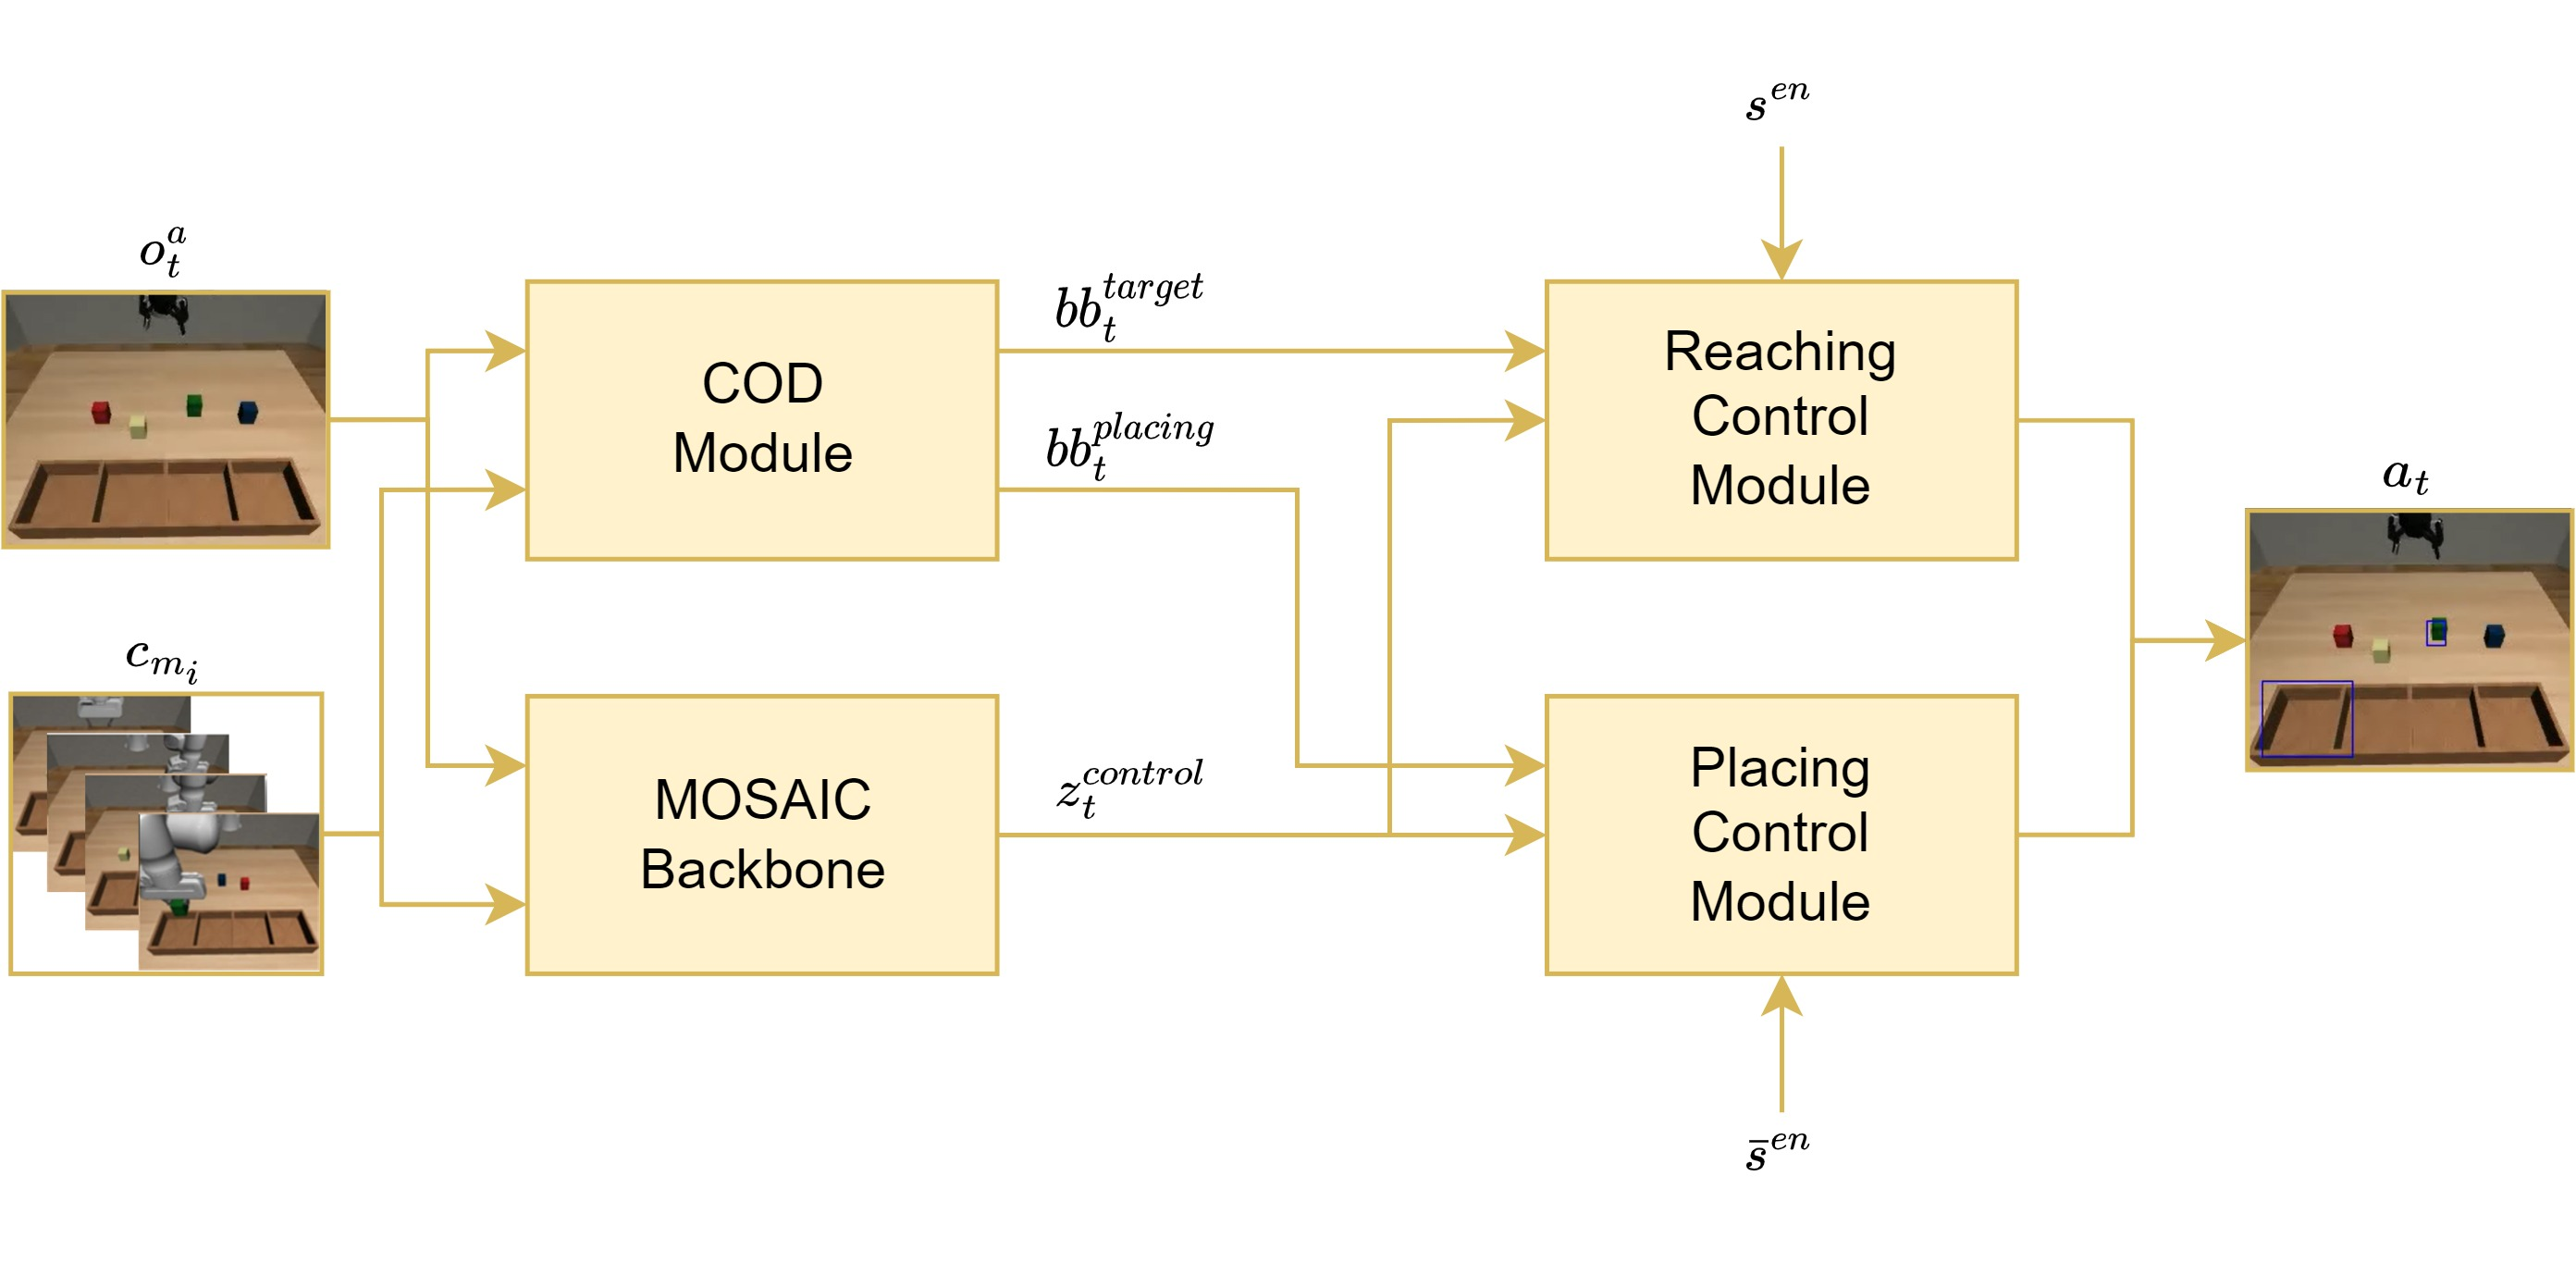
\includegraphics[width=0.9\textwidth]{figures/images/ch3/double_control_module.jpg}
    \caption{Proposed Double-Control Module Architecture. In this architecture, the Control Module is split into two distinct modules, each responsible for learning a specific primitive: the \textit{reaching} primitive and the \textit{placing} primitive. The first module takes as input the bounding box corresponding to the target object ($bb^{target}_{t}$), while the second module receives the bounding box related to the final placing location ($bb^{placing}_{t}$). This separation allows for specialized control during both the reaching and placing phases.}
    \label{fig:double_control_module}
\end{figure}
